\chapter{Podstawy teoretyczne}
\label{ch:podstawy-teoretyczne}

W niniejszym rozdziale przedstawiono zagadnienia teoretyczne, które stanowią fundament techniczny realizowanego projektu. Przedstawienie podstaw działania zastosowanych elementów pozwoli lepiej zrozumieć wyzwania projektowe oraz przyjęte metody rozwiązywania problemów związanych ze sterowaniem i kontrolą mobilnej platformy robotycznej.

Omówione zostaną najważniejsze zasady funkcjonowania enkoderów kwadraturowych, wykorzystanych do monitorowania ruchu robota - podstawowej odometrii. Zaprezentowane zostaną także zasady działania regulatora PID, powszechnie stosowanego w układach sterowania.

W dalszej części omówiono wybrane algorytmy z zakresu wizji komputerowej, takie jak detekcja krawędzi i rozpoznawanie kolorów, które stanowią istotne elementy systemu wizyjnego robota.

\section{Enkodery}
Enkodery są urządzeniami pomiarowymi, które umożliwiają śledzenie ruchu obrotowego lub liniowego. W zastosowaniach z zakresu robotyki, takich jak opisywana platforma mobilna, enkodery umożliwiają śledzenie oraz manipulowanie prędkością lub położeniem robota w przestrzeni dwuwymiarowej. Monitorowanie położenia robota za pomocą między innymi odczytów impulsów z enkoderów stanowi podstawę szerokiej dziedziny robotyki mobilnej - odometrii. W zależności od potrzeb, dodatkowym sensorem możliwym do wykorzystania jest czujnik żyroskopowy IMU (ang. \english{Inertial Measurement Unit}) - zwracający wartości przyspieszeń liniowych oraz kątowych. W tym projekcie zostały wykorzystane jedynie enkodery, ze względu na sposób poruszania się robota. 

Enkodery dzielą się na enkodery optyczne, magnetyczne i mechaniczne, w zależności od zastosowanej technologii detekcji. Szczególna uwaga zostanie poświęcona enkoderom magnetycznym umożliwiających detekcję kierunku ruchu - enkoderom kwadraturowym. 

\subsection{Rodzaje enkoderów}

Enkodery klasyfikowane są na podstawie zjawisk fizycznych wykorzystywanych do wykrywania ruchu. Główne typy to\cite{bib:enkoder-mag-opt}:

\begin{itemize}
    \item \textbf{Enkodery optyczne} - podstawę budowy stanowi przeźroczysta tarcza kodowa, przymocowana do wału silnika. Na tarczy znajdują się otwory w określonych miejscach, przez które na układ elementów światłoczułych pada wiązka światła podczerwonego generowanego przez diodę IR LED. 
    \item \textbf{Enkodery magnetyczne} - działają w oparciu o zmiany pola magnetycznego, zwykle generowanego przez magnes przymocowany do wału silnika. Zastosowanie efektu Hall' a w tych enkoderach pozwala na wykrywanie zmian w polu magnetycznym, poprzez generowanie napięcia w czujnikach Hall' a.
    \item \textbf{Enkodery mechaniczne} - najprostszy rodzaj enkoderów, wykorzystujący mechaniczne styki do generowania impulsów. Ze względu na ograniczoną trwałość są rzadziej stosowane w precyzyjnych aplikacjach.
\end{itemize}


\subsection{Efekt Hall' a}

Efekt Halla \cite{bib:zjawisko-halla} stanowi podstawę działania magnetycznych enkoderów kwadraturowych, wykorzystywanych do pomiaru prędkości i kąta położenia wałów obrotowych. Odkryty przez Edwina Halla w 1879 roku, efekt ten polega na generowaniu tzw. napięcia Halla – różnicy potencjałów w przewodniku umieszczonym w zewnętrznym polu magnetycznym, przez który przepływa prąd. Zjawisko to wynika z działania siły Lorentza na nośniki ładunku w przewodniku, kierującej je w stronę prostopadłą do kierunku przepływu prądu oraz linii pola magnetycznego.

Siła Lorentza działająca na nośniki ładunku jest opisana równaniem:
\[
\vec{F} = q \cdot (\vec{E} + \vec{v} \times \vec{B})
\]
, gdzie:
\begin{itemize}
    \item \( q \) - ładunek elektryczny nośnika prądu,
    \item \( \vec{E} \) - wektor pola elektrycznego,
    \item \( \vec{v} \) - prędkość nośnika ładunku,
    \item \( \vec{B} \) - wektor indukcji magnetycznej.
\end{itemize}

Efektem działania siły Lorentza jest przemieszczenie nośników ładunku w kierunku prostopadłym do przepływu prądu i pola magnetycznego, prowadzące do powstania napięcia Halla (\( U_H \)) w poprzek przewodnika. Wartość tego napięcia jest opisana wzorem:
\[
U_H = \frac{I B}{n \cdot q \cdot d}
\]
, gdzie:
\begin{itemize}
    \item \( I \) - natężenie prądu elektrycznego,
    \item \( B \) – indukcja magnetyczna,
    \item \( n \) – koncentracja nośników ładunku w materiale,
    \item \( d \) – grubość przewodnika.
\end{itemize}

\subsection{Enkodery kwadraturowe oparte na efekcie Halla}

Enkodery kwadraturowe są szeroko stosowane do precyzyjnego pomiaru prędkości i kąta obrotu silnika oraz umożliwiają określanie kierunku ruchu. W magnetycznych enkoderach kwadraturowych, zbudowanych w oparciu o efekt Halla, umieszcza się dwa czujniki Halla rozmieszczone pod kątem 90° względem siebie [\ref{rys2:encoders-sample}]. Podczas obrotu wału silnika wraz z magnesem, pole magnetyczne ulega zmianie wraz z obrotem, co powoduje zmiany w napięciu Halla i dalej do generowania impulsów oznaczających ruch silnika. 

Zastosowanie jednego czujnika umożliwia wykrycie ruchu oraz zliczanie ilości impulsów generowanych przez obrót. Pewnym mankamentem wykorzystania tylko jednego czujnika jest brak możliwości wykrycia kierunku obrotu. Dzięki dodaniu drugiego sensora Hall' a, kierunek ruchu można wykryć na podstawie odczytu sygnału generowanego przez enkoder, ponieważ jeden z kanałów enkodera jako pierwszy zwróci stan wysoki, co będzie oznaczało obrót w konkretną stronę. Wizualizacja sygnału generowanego przez enkoder kwadraturowy znajduje się na grafice [\ref{rys2:encoders-graf}].

Wysoka odporność na zużycie mechaniczne oraz stabilność działania w trudnych warunkach środowiskowych, takich jak wysoka wilgotność lub zapylenie, czynią magnetyczne enkodery kwadraturowe bardziej niezawodnymi niż ich optyczne odpowiedniki. Cechy te sprawiają, że magnetyczne enkodery kwadraturowe są szczególnie atrakcyjne w zastosowaniach przemysłowych oraz robotycznych, gdzie kluczowe są trwałość i precyzja.

\begin{figure}[h]
    \centering
    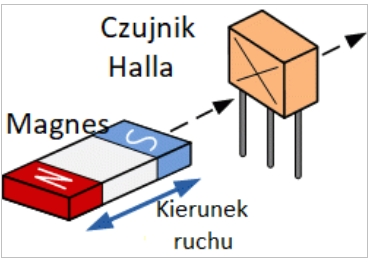
\includegraphics[width=0.5\textwidth]{./graf/halla-enc.jpg}
    \caption{Rysunek przedstawiający zasadę działania czujnika Hall' a \cite{bib:hall_net}}
    \label{rys2:encoders-graf}
\end{figure}

\begin{figure}[h]
    \centering
    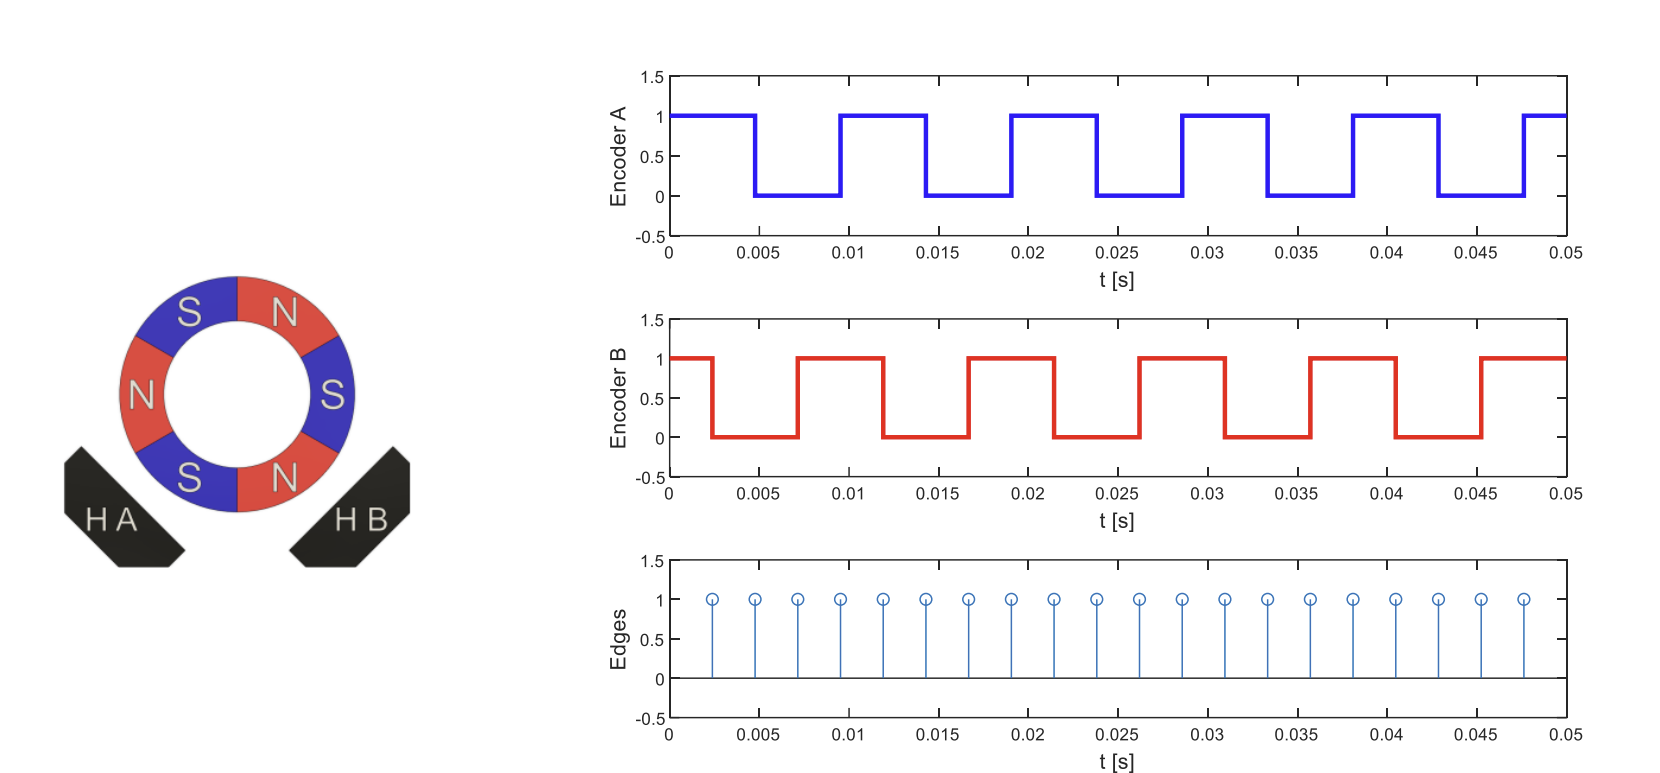
\includegraphics[width=0.8\textwidth]{./graf/enkoders.png}
    \caption{Rysunek przedstawiający ideową budowę enkodera kwadraturowego oraz sygnały przez niego generowane \cite{bib:encoders-pid}}
    \label{rys2:encoders-graf}
\end{figure}

\begin{figure}[h]
    \centering
    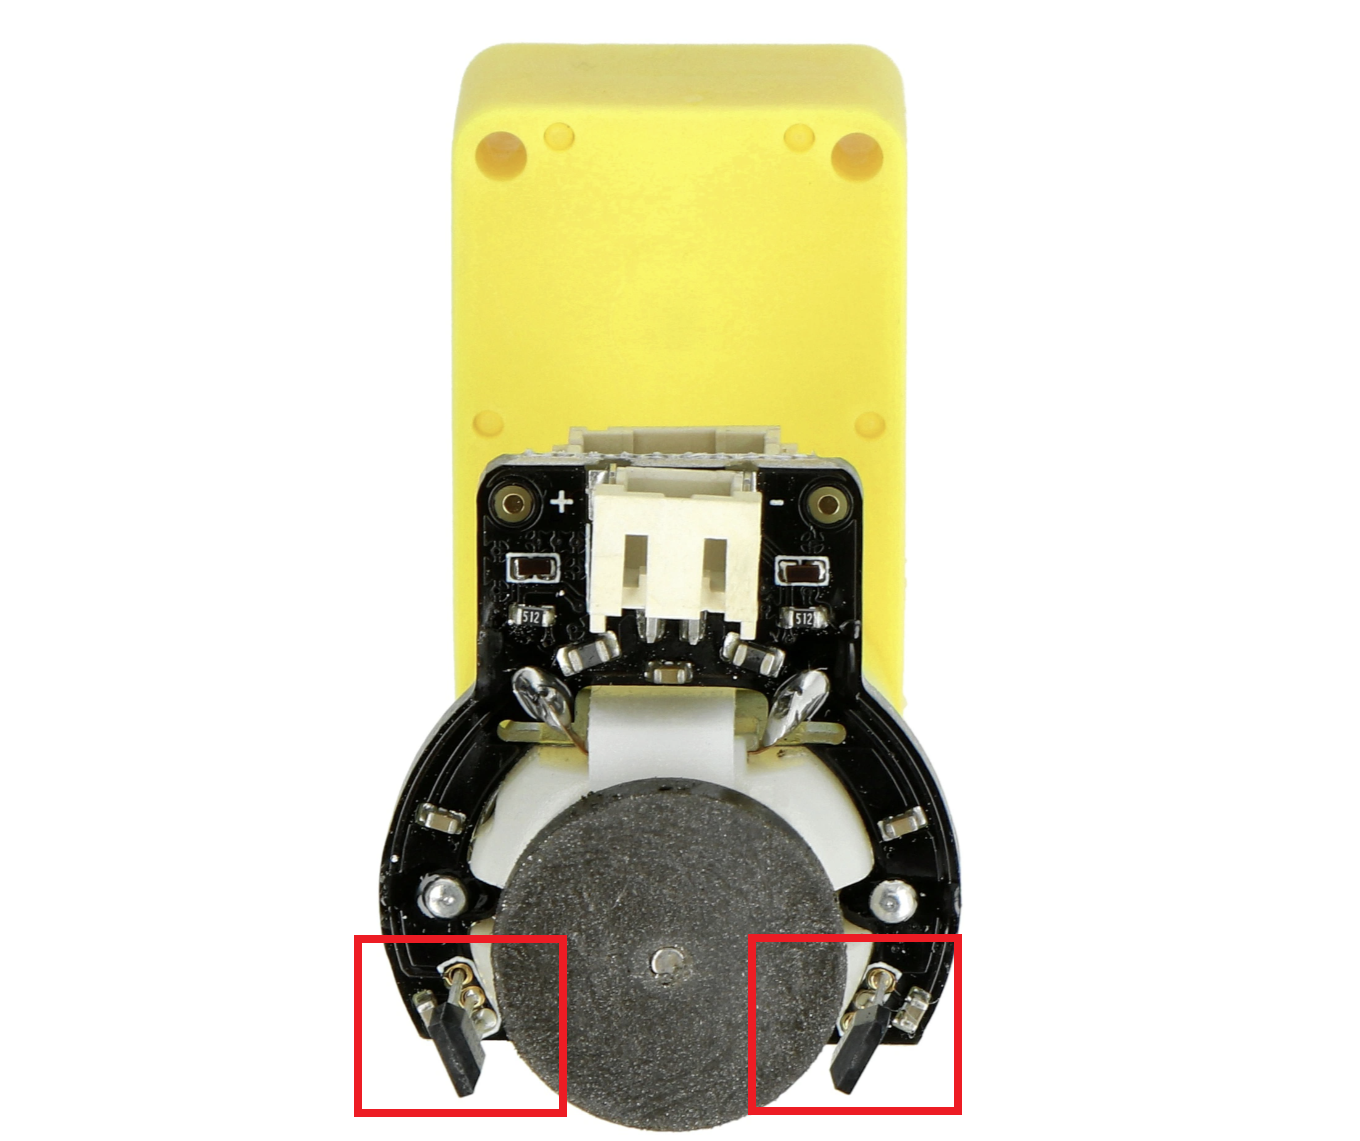
\includegraphics[width=0.5\textwidth]{./graf/enkoder-silnik.png}
    \caption{Przykładowy wygląd enkodera opartego o efekt Hall' a z oznaczonymi tranzystorami wykrywającymi zmiany pola magnetycznego podczas obrotu wału \cite{bib:botland-hall}}
    \label{rys2:encoders-sample}
\end{figure}

\clearpage

\section{Regulator PID}

Regulator PID (ang. \textit{Proportional-Integral-Derivative}) jest jednym z najczęściej stosowanych regulatorów w systemach automatycznego sterowania, ze względu na wysoką jakość regulacji gwarantującą uzyskanie zerowej wartości uchybu. Dodatkowo wykorzystanie aż trzech członów - proporcjonalnego, całkującego oraz różniczkującego, daje projektantowi duże możliwości dostosowania charakterystyki odpowiedzi czasowej regulatora, tak aby spełnić wymagania projektowe. 

\subsection{Ogólny schemat układu regulacji}

Grafika [\ref{rys2:regulacja1}] przedstawia ideowy schemat zamkniętego układu regulacji. Oznacza to, że występuje w nim pętla sprzężenia zwrotnego, a więc wartość wyjściowa zostaje dodana na wejściowy węzeł sumacyjny, w celu obliczenia uchybu. 

Wartość zadana jest kierowana na wejście regulatora, obliczającego sterowanie, które następnie jest wejściem dla urządzenia wykonawczego. Ostatnim elementem jest odczyt wartości uzyskanych i ponowne przekazanie ich na wejście układu w celu korekcji sterowania.

Na zaprezentowanym schemacie występuje również czynnik \(z(t)\), reprezentuje on zakłócenia wpływające na zachowanie wartości regulowanej. Wartość zakłócenia istotnie może zmienić wartość sterowania, która zostanie odpowiednio dostosowana poprzez regulator w celu kompensacji szumu. 

\begin{figure}[h]
    \centering
    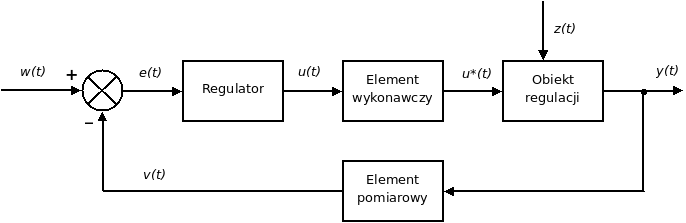
\includegraphics[width=1.0\textwidth]{./graf/regulacja1.png}
    \caption{Rysunek przedstawiający ogólny schemat układu regulacji automatycznej \cite{bib:wiki-regulacja}}
    \label{rys2:regulacja1}
\end{figure}

\subsection{Składnik proporcjonalny $P$}

Składnik proporcjonalny jest liniowo zależny od uchybu $e(t)$ i odpowiada za natychmiastową reakcję na różnicę między wartością zadaną a rzeczywistą. Działa zgodnie ze wzorem:

\begin{equation}
P(t) = K_p e(t) .
\end{equation}

Im większa wartość wzmocnienia proporcjonalnego $K_p$, tym regulator bardziej dynamicznie reaguje na uchyb, co przyspiesza osiągnięcie wartości zadanej, ale przy zbyt dużych wartościach może prowadzić do przeregulowania, a w konsekwencji oscylacji.

\subsection{Składnik całkujący $I$}

Składnik całkujący sumuje wartości uchybu w czasie, co pozwala na eliminację uchybu ustalonego – różnicy między wartością zadaną a rzeczywiście uzyskaną w stanie ustalonym.

\begin{equation}
    e_u = \lim_{t \to \infty} e(t)
    \label{eq:lim_stab}
\end{equation}
, gdzie:
\begin{itemize}
    \item $e_u$ - uchyb w stanie ustalonym,
    \item $e(t)$ - funkcja wiążąca wartość uchybu z czasem
\end{itemize}

Dla stabilnych układów dynamicznych wartość uchybu w granicy, gdzie czas dąży do nieskończoności, osiąga wartość stałą. Im jest mniejsza, tym jakość regulacji jest bardziej dokładna. 

\hspace{1cm}

Składnik całkujący jest dany równaniem:
\begin{equation}
I(t) = K_i \int_{0}^{t} e(\tau) d\tau .
\end{equation}

Dzięki temu składnikowi, regulator PID potrafi zniwelować długotrwały uchyb, chociaż przy zbyt dużych wartościach wzmocnienia $K_i$ może wystąpić zjawisko przeregulowania oraz niestabilności układu.

\subsection{Składnik różniczkujący $D$}

Składnik różniczkujący uwzględnia szybkość zmian uchybu $e(t)$, co pozwala na szybsze reagowanie na gwałtowne zmiany i przeciwdziałanie efektowi przeregulowania. Opisuje go wyrażenie:

\begin{equation}
D(t) = K_d \frac{de(t)}{dt} .
\end{equation}

Ten składnik regulatora poprawia stabilność i tłumi oscylacje, jednak zbyt duża wartość wzmocnienia $K_d$ może prowadzić do niestabilności układu, zwłaszcza w obecności szumów.

\subsection{Pełne równanie regulatora PID}

Łącząc wszystkie trzy składniki, równanie regulatora PID przyjmuje postać:

\begin{equation}
u(t) = K_p e(t) + K_i \int_{0}^{t} e(\tau) d\tau + K_d \frac{de(t)}{dt}
\end{equation}

, gdzie:
\begin{itemize}
    \item $K_p e(t)$ – składnik proporcjonalny, który odpowiada za szybką reakcję na zmiany,
    \item $K_i \int_{0}^{t} e(\tau) d\tau$ – składnik całkujący, który eliminuje uchyb statyczny,
    \item $K_d \frac{de(t)}{dt}$ – składnik różniczkujący, który przeciwdziała nagłym zmianom uchybu.
\end{itemize}

Często ze względu na relatywnie prostsze obliczenia, szczególnie podczas analizy stabilności oraz wyznaczania charakterystyk dynamicznych stosuje się postać operatorową (przekształcając równanie w postaci czasowej za pomocą operatora Laplace’a [\mathcal{L}]) regulatora PID. 

\begin{equation}
    U(s) = (K_p + \frac{K_i}{s} + K_d s) E(s)
\end{equation}

, gdzie:
\begin{itemize}
    \item $E(s)$ - uchyb w dziedzinie operatorowej,
    \item $K_p, K_i, K_d$ wartości wzmocnienień odpowiednich członów.
\end{itemize}


Regulacja parametrów $K_p$, $K_i$ i $K_d$ pozwala na dostosowanie charakterystyki regulatora PID do specyfiki sterowanego obiektu. Optymalne wartości tych parametrów zazwyczaj są dobierane metodą prób i błędów lub za pomocą metod takich jak strojenie Zieglera-Nicholsa.

\subsection{Działanie regulatora PID}

Działanie regulatora PID opiera się na przetwarzaniu sygnału uchybu $e(t)$, różnicy między wartością zadaną $y_{set}$ a wartością rzeczywistą $y(t)$ wielkości regulowanej:

\begin{equation}
e(t) = y_{set} - y(t) .
\end{equation}

Uchyb jest jednym z podstawowych wskaźników jakości regulacji, określający jak dobrze wybrany regulator uzyskuje wartość zadaną. Cechą charakterystyczną regulatora PID jest całkowita skuteczność uzyskania uchybu równego zero dla stabilnych układów dynamicznych. Zastosowanie innych regulatorów takich jak P (z jedynie członem proporcjonalnym) lub PI (z członem proporcjonalnym i drugim 
członem całkującym) nie gwarantuje uzyskania uchybu równego zero. 


\subsection{Zastosowanie regulatora PID w sterowaniu robotem mobilnym}

W omawianym projekcie regulator PID znajduje zastosowanie w kontrolowaniu odległości jaką pokonuje platforma mobilna poprzez odpowiednie sterowanie napięciem zasilania elementów wykonawczych. Nastawy regulatora zostały dostosowane metodą prób i błędów. Uzyskana jakość regulacji jest wystarczająca do spełnienia wymagań projektowych. 

\section{Napęd różnicowy}

Napęd różnicowy jest często stosowanym rozwiązaniem w robotach mobilnych do wielu zastosowań, ze względu na stosunkową prostą konstrukcję oraz duże możliwości ruchu.  Konstrukcja napędu składa się z dwóch niezależnie napędzanych kół, umieszczonych po przeciwnych stronach osi robota. Dodatkowym elementem konstrukcyjnym może być jedno lub więcej biernych kół podporowych, zapewniających lepszą stabilność platformy - w przypadku poniższego projektu zostały zastosowane dwa elementy bierne podporowe. 

\subsection{Kinematyka napędu różnicowego}

Model kinematyczny napędu różnicowego opisuje związek między prędkościami kół a ruchem platformy w przestrzeni dwuwymiarowej. W przypadku idealnym zakładającym brak poślizgu kół oraz brak luzów na przekładni, prędkość liniowa platformy \(\upsilon\) oraz prędkość kątowa \(\omega\) wyrażają się równaniami [\ref{eq:linear}].

\begin{equation}
    \centering
    \upsilon = \frac{\upsilon_r + \upsilon_l}{2},  \omega = \frac{\upsilon_r + \upsilon_l}{b}
    \label{eq:linear}
\end{equation}

, gdzie:
\begin{itemize}
    \item \(\upsilon_r\) oraz \(\upsilon_l\) to prędkości odpowiednio prawego oraz lewego koła,
    \item \(b\) oznacza odległość pomiędzy osiami kół.
\end{itemize}

W bazowym układzie współrzędnych przemieszczenie robota opisują równania [\ref{angular}]:

\begin{equation}
    \centering
    \dot{x} = \upsilon cos(\theta), \dot{y} = \upsilon sin(\theta), \dot(\theta) = \omega
    \label{eq:angular}
\end{equation}

, gdzie:
\begin{itemize}
    \item \(x\) i \(y\) - współrzędne środka masy w układzie współrzędnych odniesienia
    \item \(\theta\) - orientacja platformy.
\end{itemize}

\clearpage

\begin{figure}[h!]
    \centering
    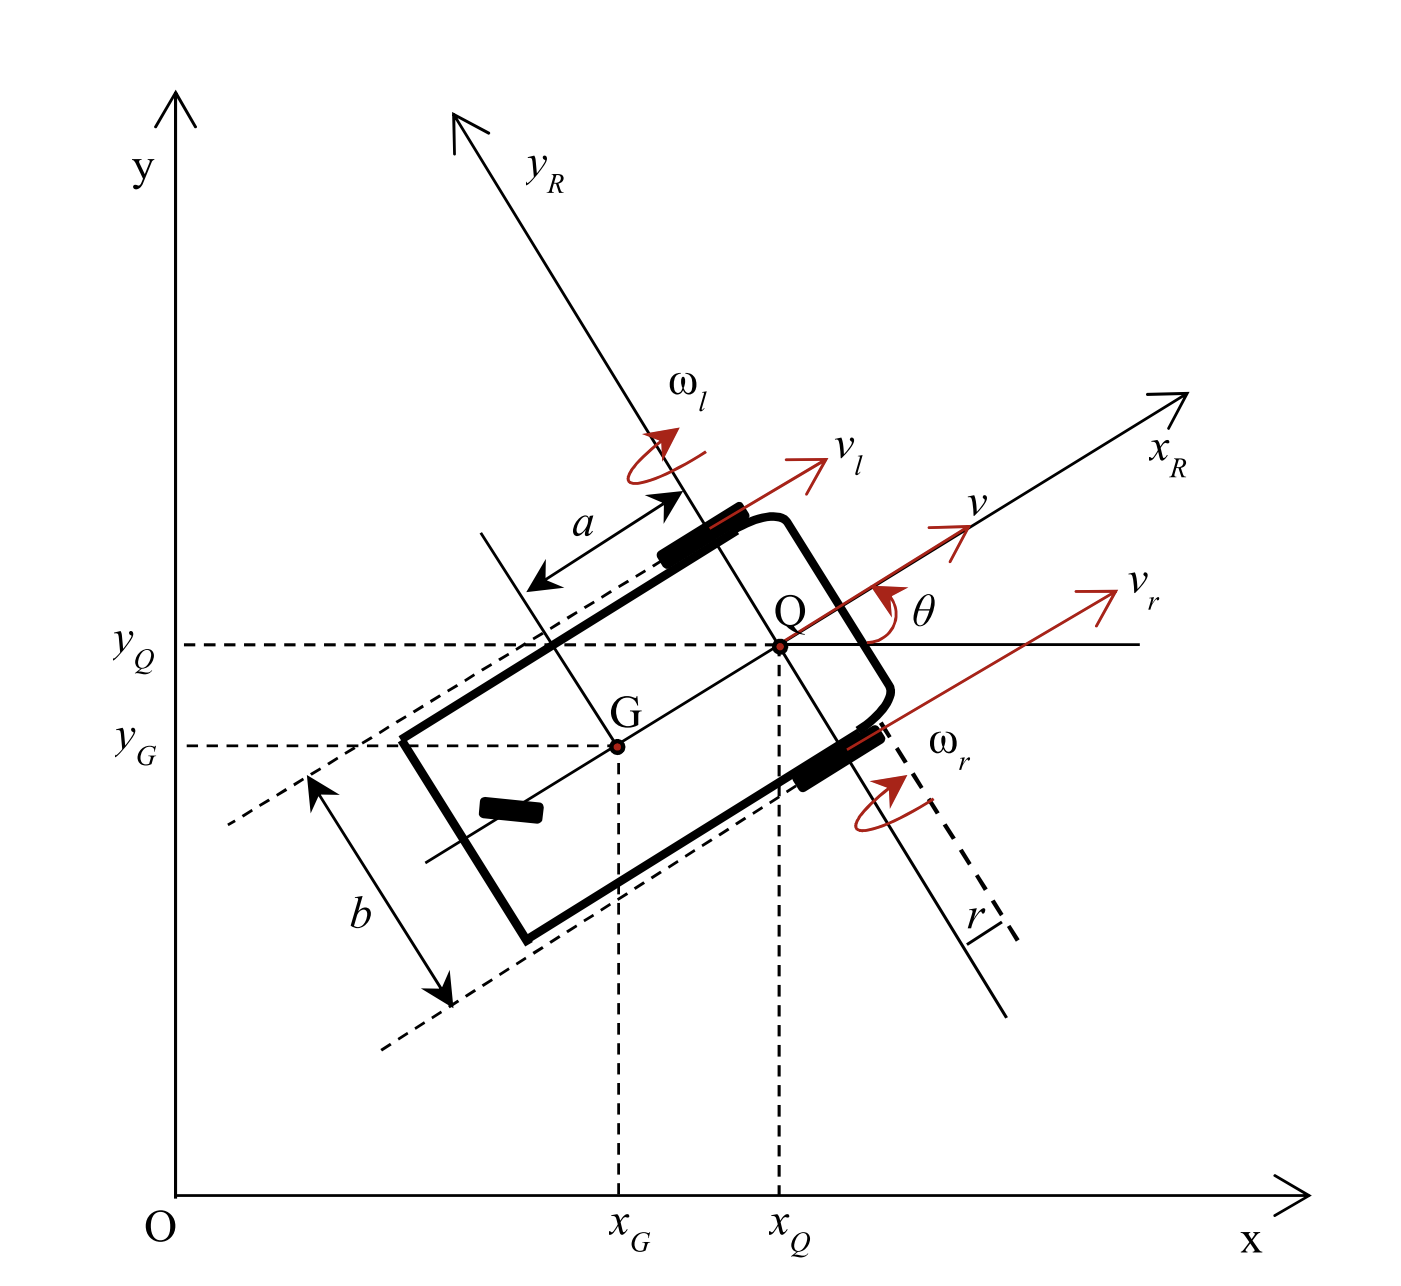
\includegraphics[width=0.7\textwidth]{./graf/diff-drive.png}
    \caption{Grafika stanowiąca wizualizację przekształceń kinematyki robota \cite{bib:konferencja}}
\end{figure}

\section{Odometria - metoda przyrostowa}

Odometria jest metodą znaną od lat, mimo to nadal szeroko stosowaną jako metodę nawigacji w robotyce mobilnej. Cechuje się dobrą dokładnością w krótkim oknie czasowym oraz relatywnie niską ceną wdrożenia. Podstawą odometrii jest całkowanie (sumowanie) przyrostowej informacji pozyskanej na przykład z enkoderów inkrementalnych (przyrostowych) zamontowanych na napędzie, w czasie. Może to prowadzić do dużej akumulacji błędów w przypadku szerokiego okna czasowego, a tym samym do znacznej zmiany orientacji robota względem założonej. Mimo to, metoda ta jest szeroko stosowana, między innymi w połączeniu z innymi metodami orientacji  robota w przestrzeni w celu eliminacji nagromadzonych błędów. 

\hspace{1cm}

Aby wyznaczyć, ile impulsów należy zliczyć w celu wykonania określonego przemieszczenia względem układu bazowego, należy skorzystać ze wzoru \ref{eq:impulsy}, a następnie \ref{eq:impulsy-odl}.

\begin{equation}
    \centering
    c_m = \pi \frac{D_n}{n C_e}
    \label{eq:impulsy}
\end{equation}
, gdzie:
\begin{itemize}
    \item \(c_m\) - współczynnik przeliczenia impulsów licznika na przebytą odległość,
    \item \(D_n\) - nominalna średnica kół,
    \item \(C_e\) - rozdzielczość licznika w impulsach na obrót,
    \item \(n\) - współczynnik biegu - przeliczenie obrotów silnika na obroty kół.
\end{itemize}

\begin{equation}
    \centering
    \Delta U_{R/L, I} = c_m N_{R/L, I}
    \label{eq:impulsy-odl}
\end{equation}
, gdzie:
\begin{itemize}
    \item \(\Delta U_{R/L, I}\) - przebyta odległość,
    \item \(c_m\) -  współczynnik przeliczenia impulsów licznika na przebytą odległość,
    \item \(N_{R/L, I}\) - ilość zliczonych impulsów przez enkodery koła prawego (R) oraz lewego (L) w krótkim czasie \(I\). 
\end{itemize}

\section{Podstawy wykrywania krawędzi w wizji komputerowej}

Wykrywanie krawędzi to jedna z podstawowych technik przetwarzania obrazów stosowana w wizji komputerowej, umożliwiająca ekstrakcję istotnych informacji strukturalnych z obrazu. Proces ten polega na detekcji nagłych zmian intensywności pikseli, które odpowiadają krawędziom obiektów w przestrzeni obrazu. Krawędzie dostarczają kluczowych danych o kształtach i konturach obiektów, wspomagając zadania takie jak segmentacja obrazu, rozpoznawanie obiektów oraz analiza ruchu. Wysoka jakość detekcji krawędzi jest zatem niezbędna dla dokładności i skuteczności systemów wizji komputerowej.

Jednym z najbardziej uznanych algorytmów wykrywania krawędzi jest metoda Canny'ego, opracowana przez Johna F. Canny’ego w 1986 roku. Algorytm ten jest ceniony za swoje właściwości w zakresie selektywnej detekcji krawędzi przy jednoczesnym tłumieniu szumów, co zapewnia spójną i wyraźną detekcję konturów.

\subsection{Algorytm Canny’ego}

Algorytm Canny’ego \cite{bib:canny-article} to złożona metoda wieloetapowa, której celem jest precyzyjna detekcja krawędzi przy minimalnym wpływie szumów. Składa się on z pięciu kluczowych etapów:

\begin{enumerate}
    \item \textbf{Wygładzanie} (ang. \textit{Smoothing}): W celu redukcji wpływu szumów obraz jest najpierw poddawany filtracji za pomocą splotu z maską Gaussa, co pozwala na zachowanie istotnych struktur obrazu przy jednoczesnym tłumieniu drobnych zaburzeń. Przykładowa maska Gaussa o rozmiarze \(3 \times 3\) ma postać:

    \[
    G = \begin{bmatrix}
    \frac{1}{16} & \frac{1}{8} & \frac{1}{16} \\
    \frac{1}{8} & \frac{1}{4} & \frac{1}{8} \\
    \frac{1}{16} & \frac{1}{8} & \frac{1}{16}
    \end{bmatrix}
    \]

    \item \textbf{Obliczanie gradientu}: Po wygładzeniu obrazu przeprowadza się obliczenia gradientu intensywności dla każdego piksela, co pozwala na identyfikację miejsc o gwałtownych zmianach intensywności. Gradient jest obliczany w kierunkach poziomym (za pomocą maski Sobela \(S_x\)) i pionowym (za pomocą maski Sobela \(S_y\)):

    \[
    S_x = \begin{bmatrix}
    -1 & 0 & 1 \\
    -2 & 0 & 2 \\
    -1 & 0 & 1
    \end{bmatrix}, \quad 
    S_y = \begin{bmatrix}
    1 & 2 & 1 \\
    0 & 0 & 0 \\
    -1 & -2 & -1
    \end{bmatrix}
    \]

    Na tej podstawie wyznaczana jest wielkość gradientu \(G\):

    \[
    G = \sqrt{G_x^2 + G_y^2}
    \]

    oraz jego kierunek:

    \[
    \Theta = \text{atan2}(G_y, G_x)
    \]

    \item \textbf{Tłumienie nie-maksymalne} (ang. \textit{Non-maximum suppression}): W tym etapie algorytm identyfikuje i zachowuje jedynie lokalne maksima gradientu w kierunku krawędzi, co pozwala na wyostrzenie konturów krawędzi i eliminację nieistotnych pikseli, które nie leżą na krawędzi obiektów.

    \item \textbf{Podwójne progowanie} (ang. \textit{Double thresholding}): Po wstępnej selekcji krawędzi, algorytm wprowadza dwa progi — wysoki i niski. Piksele o wartości gradientu przekraczającej wysoki próg uznaje się za pewne krawędzie, podczas gdy piksele o wartościach poniżej niskiego progu są eliminowane. Piksele mieszczące się pomiędzy progami są klasyfikowane jako krawędzie słabe, które wymagają dalszej analizy.

    \item \textbf{Śledzenie krawędzi z histerezą} (ang. \textit{Edge tracking by hysteresis}): W końcowym kroku algorytm wykonuje śledzenie połączonych pikseli, aby zachować spójność krawędzi. Piksele oznaczone jako krawędzie słabe są akceptowane jako część krawędzi tylko wtedy, gdy są połączone z krawędziami silnymi. Ten proces zapobiega przypadkowej detekcji krawędzi i pozwala na eliminację fragmentarycznych lub pojedynczych pikseli wynikających z szumu.
\end{enumerate}


\begin{figure}[h!]
    \centering
    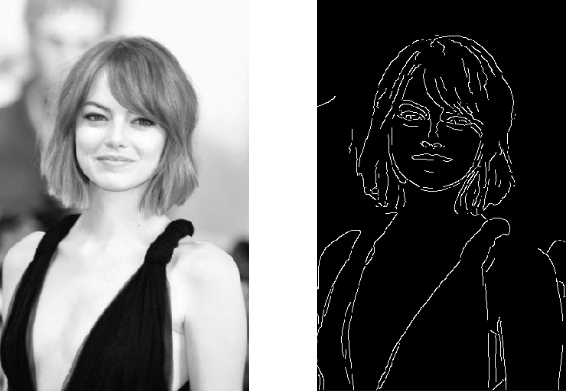
\includegraphics[width=0.6\textwidth]{./graf/canny-edge.png}
    \caption{Zdjęcie przedstawiające skuteczność wykrywania krawędzi algorytmem Canny'ego}
\end{figure}

\clearpage

\section{Podstawy rozpoznawania kolorów w wizji komputerowej}

Istotnym elementem wizji komputerowej jest możliwość rozpoznawania kolorów. Funkcjonalność ta jest szczególnie przydatna w automatyce, robotyce oraz w metodach sztucznej inteligencji. Pozwala na klasyfikację obiektów przy pomocy prostych algorytmów analizy wizyjnej, jak ma to miejsce w przypadku tego projektu, ale również jest częścią zaawansowanego trenowania sieci neuronowych, tym samym umożliwiając bardzo dokładną klasyfikację obiektów o różnym kształcie i kolorze. 

W tej sekcji omówione zostaną podstawowe zasady oraz techniki wykorzystywane w procesie rozpoznawania kolorów.


\subsection{Teoria koloru}

Kolor jest wynikiem interpretacji długości fali światła przez ludzki wzrok. W systemach wizyjnych kolor jest reprezentowany za pomocą modeli kolorów, które pozwalają na matematyczną reprezentację informacji o barwie i jej intensywności. Najczęściej stosowane modele kolorów to przestrzenie RGB (ang. \textit{Red, Green, Blue}), HSV (ang. \textit{Hue, Saturation, Value}) oraz YCrCb (ang. \textit{Luminance, Chrominance}).

\begin{itemize}
    \item \textbf{Model RGB} [\ref{rys2:rgb1}] — Kolory reprezentowane są jako kombinacja trzech składowych: czerwonej, zielonej i niebieskiej. Jest to podstawowy model stosowany w systemach cyfrowych do rejestrowania i wyświetlania obrazów.
    \item \textbf{Model HSV} [\ref{rys2:hsv1}]— Przestrzeń HSV, zdefiniowana przez odcień, nasycenie i jasność, jest bardziej zbliżona do ludzkiego postrzegania kolorów. Pozwala ona na łatwiejsze odróżnianie odcieni niezależnie od zmian oświetlenia, co czyni ją szczególnie przydatną w detekcji kolorów w wizji komputerowej.
    \item \textbf{Model YCrCb} [\ref{rys2:ycrcb1}]— Oddziela jasność (luminancję) od informacji o kolorze (chrominancję). Ta przestrzeń kolorów jest powszechnie stosowana w kompresji obrazu i w systemach przetwarzania obrazu, gdyż zapewnia stabilność kolorów przy zmiennych warunkach oświetleniowych.
\end{itemize}


\subsection{Proces rozpoznawania kolorów}
Proces rozpoznawania kolorów obejmuje szereg etapów pozwalających na identyfikację pikseli o określonych wartościach kolorystycznych. Wyróżnić można następujące kroki:

\begin{enumerate}
    \item \textbf{Przechwytywanie obrazu} — Obraz jest rejestrowany przy pomocy kamery, która przekazuje dane w formacie cyfrowym.
    \item \textbf{Przetwarzanie obrazu} — Obraz przechodzi przez operacje wstępnego przetwarzania, takie jak filtrowanie i segmentacja, aby wyodrębnić istotne informacje kolorystyczne.
    \item \textbf{Ekstrakcja cech} — Analizowane są wartości kolorystyczne pikseli, co umożliwia identyfikację obiektów na podstawie ich kolorów.
    \item \textbf{Decyzja} — Na podstawie zebranych informacji o kolorze podejmowana jest decyzja o klasyfikacji obiektów.
\end{enumerate}

\subsection{Algorytmy rozpoznawania kolorów}

W literaturze przedmiotu występuje wiele podejść do rozpoznawania kolorów, takich jak analiza histogramu, segmentacja obrazu oraz analiza cech. Histogramy kolorów pozwalają na szybkie określenie dominujących kolorów na obrazie, co może być użyteczne w aplikacjach czasu rzeczywistego. Segmentacja obrazu natomiast umożliwia wyodrębnienie obiektów o określonym kolorze, co może być realizowane przy pomocy algorytmów takich jak \english{k-means clustering} lub metoda \english{watershed}.


\begin{figure}[h!]
    \centering
    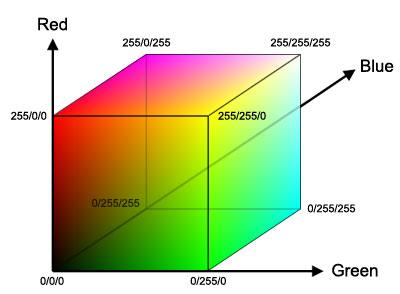
\includegraphics[width=0.6\textwidth]{./graf/rgb-model.png}
    \caption{Wizualizacja przestrzeni kolorów RGB \cite{bib:rgb-model}}
    \label{rys2:rgb1}
\end{figure}

\begin{figure}[h!]
    \centering
    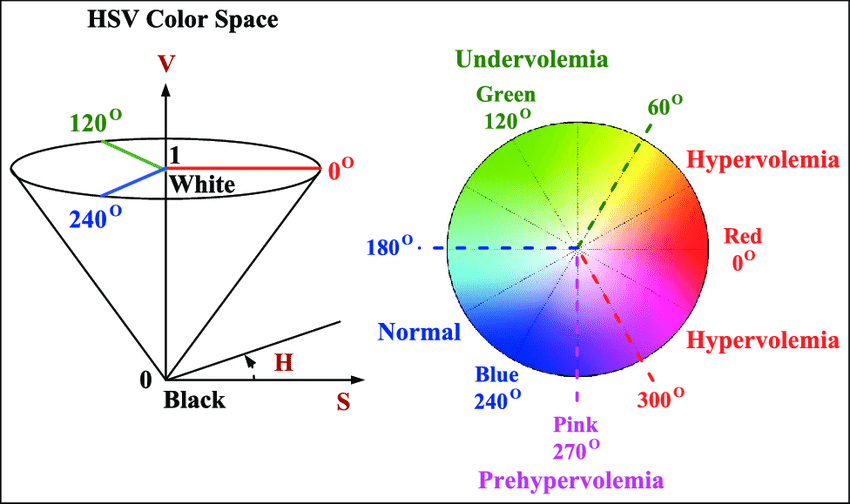
\includegraphics[width=0.6\textwidth]{./graf/hsv-model.png}
    \caption{Wizualizacja przestrzeni HSV \cite{bib:hsv-model}}
    \label{rys2:hsv1}
\end{figure}

\begin{figure}[h!]
    \centering
    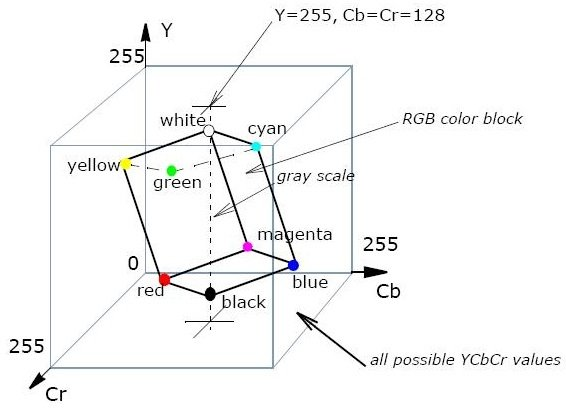
\includegraphics[width=0.6\textwidth]{./graf/ycrcb-model.png}
    \caption{Wizualizacja przestrzeni YCrCb \cite{bib:ycrcb-model}}
    \label{rys2:ycrcb1}
\end{figure}


% \subsection{Stabilność układów dynamicznych}
% \label{sek:stab}

% Stabilność układów dynamicznych jest kluczowym zagadnieniem podczas projektowania układu regulacji. W analizie stabilności sprawdza się, czy układ dąży do stanu równowagi - minimalizuje uchyb, aby fianlnie osiągnąć wartość minimalną, w przypadku regulatora PID jest to zero. W przypadku układów niestabilnych, wartość uchybu dąży do nieskończoności, co jest szczególnie nieporządane podczas projektowania rzeczywistych układów, ze względu na możliwe uszkodzenie elementów wykonawczych poprzez podanie na ich wejście zbyt dużych wartości napięcia, prądu. 

% W przypadku regulatora PID analiza stabilności opiera się wyznaczeniu charakterystyk dla zadanych nastaw - wartości parametrów wzmocnienia $K_p$, $K_i$, $K_d$. Najczęściej w celu weryfikacji stabilności układów stosuje się metody:
% \begin{itemize}
%     \item \textbf{Kryterium Hurwitza} – bazuje na analizie współczynników charakterystycznych układu dynamicznego w dziedzinie operatora Laplace’a. Metoda polega na ocenie znaku podwyznaczników macierzy Hurwitza, aby określić, czy wszystkie pierwiastki wielomianu charakterystycznego mają część rzeczywistą mniejszą od zera.
%     \item \textbf{Kryterium Nyquista} – metoda graficzna oparta na analizie funkcji transmitancji układu na wykresie Nyquista. Kryterium to bada, jak charakterystyka amplitudowo-fazowa zamkniętego układu reaguje na różne częstotliwości sygnału wejściowego. Wykres Nyquista pozwala ocenić stabilność systemu poprzez obserwację, czy jego kontur w dziedzinie częstotliwości otacza określony punkt krytyczny. Kryterium Nyquista nadaje się szczególnie do badania stabilności układów nieliniowych i bardziej złożonych systemów z opóźnieniami.
% \end{itemize}

% Teoretyczna analiza stabilności jest punktem wyjścia przy projektowaniu regulatorów PID, ponieważ zbyt duże wartości parametrów $K_p$, $K_i$, lub $K_d$ mogą prowadzić do niestabilnych oscylacji. Przykładowo, wysoka wartość wzmocnienia proporcjonalnego $K_p$ zwiększa szybkość reakcji układu, ale zbyt duża może powodować oscylacje wokół wartości zadanej. Z kolei nadmierne wzmocnienie członu różniczkującego $K_d$ prowadzi do niestabilności w obecności szumu. Metody Hurwitza i Nyquista pomagają przewidzieć te reakcje i dobrać parametry regulatora tak, aby uzyskać stabilność i oczekiwane właściwości dynamiczne układu.